\section{Probleme}

\subsection{Datenstruktur der Statusstruktur}
\label{tree}
Die von van Kreveld vorgeschlagene Datenstruktur eines balancierten binären Baums ist in dieser Form noch nicht in Java 1.8 vorhanden. Daher mussten 
wir diese selbst implementieren.
Van Kreveld schlägt einen balancierten Binärbaum vor, der nur in den Blattknoten Pixel abspeichert
und in jedem inneren Knoten $v$ die maximale Steigung aller Blätter des Teilbaums mit Wurzel $v$ speichert.
Java stellt zwar balancierte Binärbäume zur Verfügung, allerdings können diese weder augmentiert werden,
noch speichern diese ihre Elemente ausschließlich in den Blattknoten.
Deshalb haben wir die Statusstruktur basierend auf Code für einen Rot-Schwarz-Baum im Java Development Kit (TreeMap.java) implementiert.
Sie stellt einen Rot-Schwarz-Baum dar, der -- im Gegensatz zu van Krevelds Vorschlag -- in \emph{jedem} Knoten einen Pixeleintrag abspeichert
und jeden Knoten $v$ um dessen Steigung (slope) und die maximale Steigung (maxSlope) aller Nachfahrknoten augmentiert.
Bereitgestellt werden die Methoden \verb|insert(HeightedPoint pt)|, \verb|delete(HeightedPoint pt)| und \verb|isVisible(HeightedPoint pt)|,
die die Operationen implementieren, die bei den Ereignissen \verb|IN|, \verb|OUT| beziehungsweise \verb|CENTER| ausgeführt werden.
Innerhalb der Statusstruktur sind die Pixel nach ihrer Distanz zum Standpunkt georgnet.
Weil in der Statusstruktur genau die Pixel gehalten werden, die auf der Sichtlinie liegen, bedeutet dies,
dass alle Pixel, die die Sicht auf einen bestimmten verdecken können, links diesen Pixels in dem Baum liegen.
Die Methode \verb|isVisible(HeightedPoint pt)| muss also nur logaritmisch viele Vergleiche durchführen, siehe Abbildung~\ref{fig:isVisible}.

\begin{figure}[ht]
    \centering
    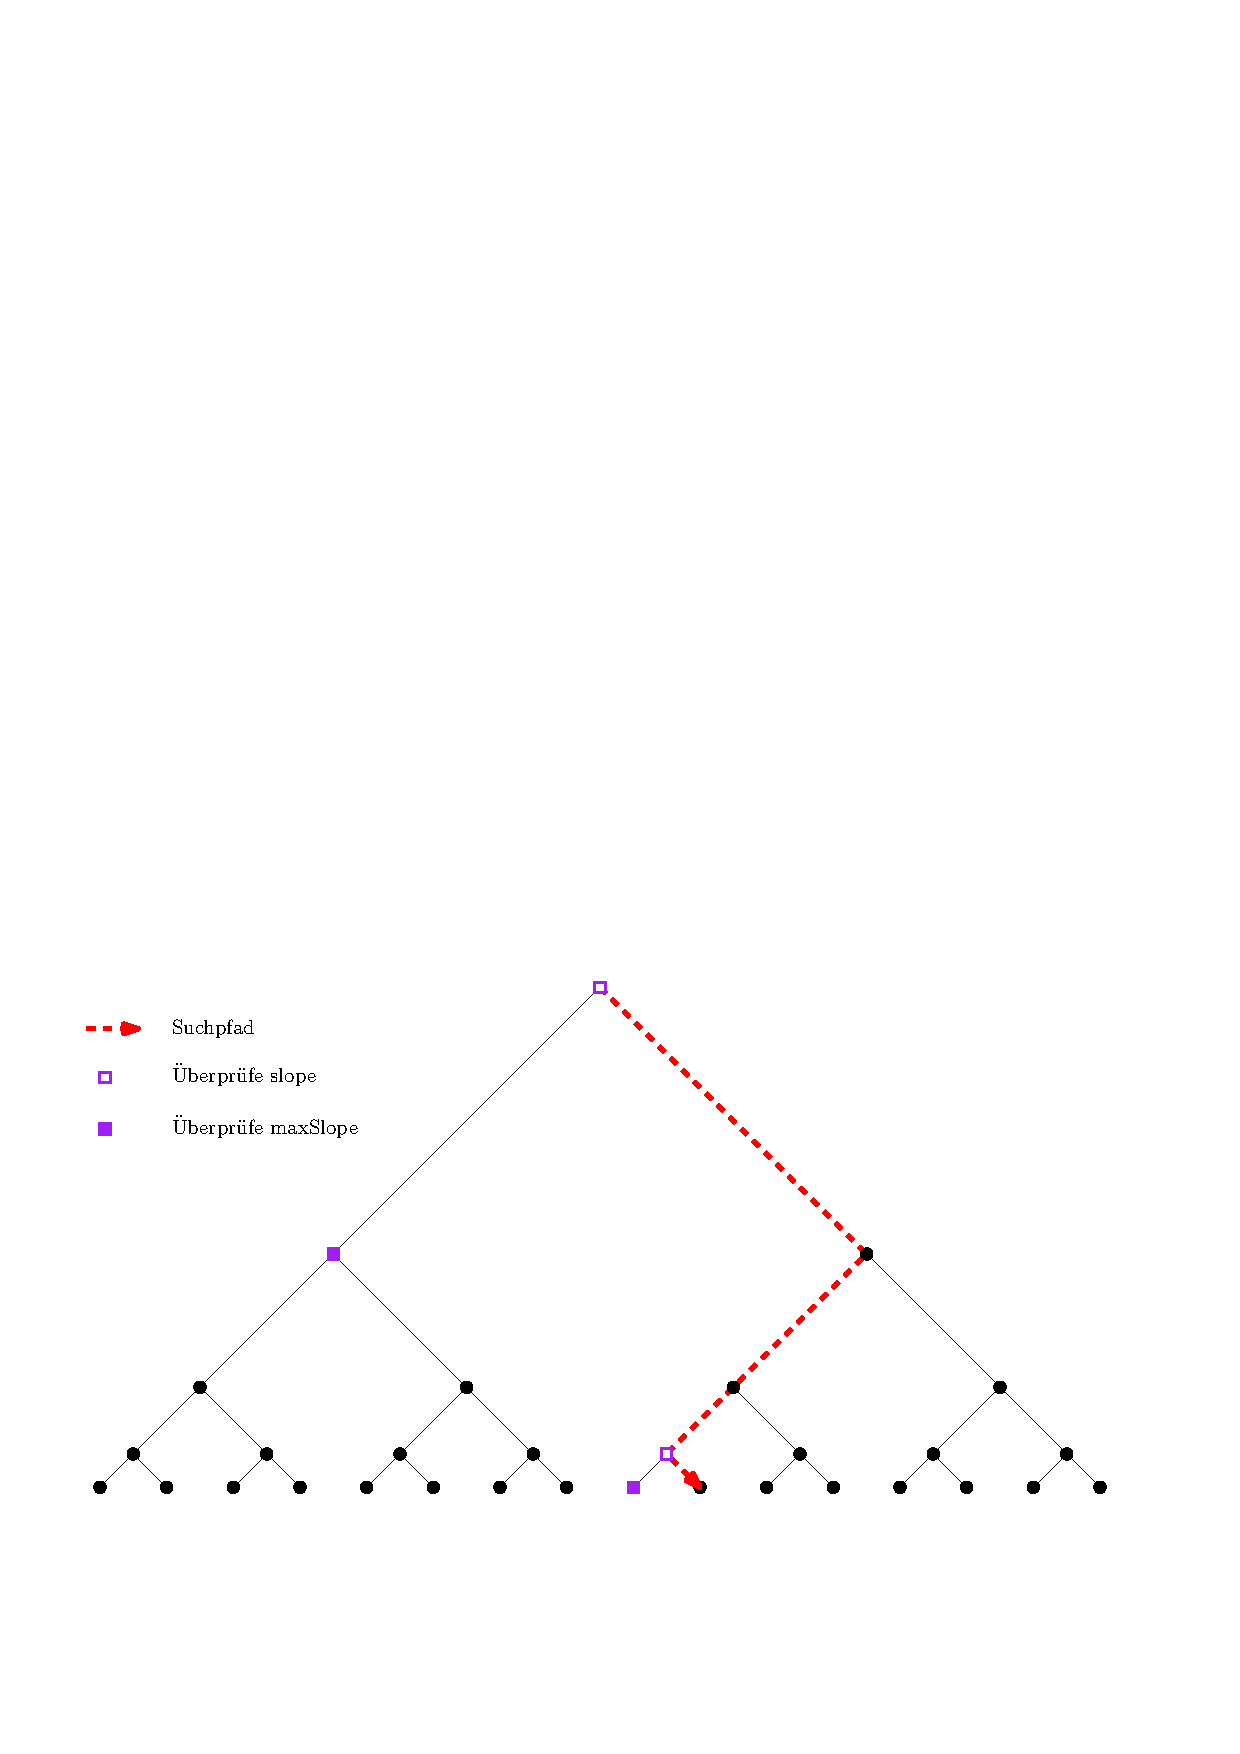
\includegraphics[width=.7\textwidth]{bilder/StatusStructure_isVisible}
    \caption[StatusStructure.isVisible(HeightedPoint pt)]{StatusStructure.isVisible(HeightedPoint pt): Die Steigung des gesuchten Punktes~pt muss mit der Steigung aller weiter links liegenden Punkte verglichen werden.}
    \label{fig:isVisible}
\end{figure}

\subsection{Speicherbedarf und Laufzeit}
\label{speicher}

Wie bereits am Ende von Kapitel \ref{sweep_adjust} erwähnt, hat die erste von uns implementierte Version des van Kreveld-Algorithmus eine 
wesentlich schlechtere Laufzeit als die des naiven Algorithmus. Durch entsprechende Tests wurde deutlich, dass bei van Krevelds Algorithmus vor allem
der Speicherbedarf eine große Rolle spielt und schnell war eines der Probleme identifiziert: die event list. Am Anfang des Programms wird die event list 
mit allen Eventtypen aller Pixel befüllt und enthält dadurch insgesamt $n \cdot n \cdot 3$ Elemente. Je größer das DEM nun ist, umso mehr Elemente 
umfasst die event list und umso mehr Speicher wird benötigt. So werden beispielsweise für ein DEM von 500x1000 Pixeln 1,5 Millionen Werte 
gleichzeitig im Speicher gehalten, was zu einer enormen Verlängerung der Laufzeit führt. 

Durch die folgenden drei Überlegungen können wir die Laufzeit des van Kreveld-Algorithmus deutlich verbessern.

\subsubsection{Verkleinern der event list}
\label{ev_klein}
Die Idee zur Verkleinerung der event list ist die folgende: Um einen enormen Speicherbedarf zu verhindern, wird die event list zu Beginn nicht mit 
allen Werten befüllt, sondern sie enthält nur die für die aktuelle Berechnung notwendigen events. Nach jeder Berechnung wird die event list dann 
aktualisiert. 

\begin{figure}[!ht]
 \centering
 \begin{BVerbatim}
  Initialisiere die Statusstruktur 
  Fülle die event list mit den auf der sweep line enthaltenen Pixeln 
  Solange die event list noch nicht leer ist 
    Do Nimm das erste event aus der Liste 
      Falls Typ == EventType.IN
	  füge Pixel in die Statusstruktur ein
      Falls Typ == EventType.OUT
	  lösche Pixel in der Statusstruktur 
      Falls Typ == EventType.CENTER
	  berechne die Sichtbarkeit des Pixels mit Hilfe der in der Statusstruktur 
	  gespeicherten Daten
      Berechne für den Pixel des events alle benachbarten Pixel 
	  Falls ein Nachbarpixel noch nicht in die event list eingefügt wurde
	       füge seine events in die event list ein
    EndDo

 \end{BVerbatim}
 \caption{Pseudocode für van Kreveld-Algorithmus mit verbesserter event list}
 \label{pseudo_krev_ev_klein}
\end{figure}

Wie aus dem Pseudocode in Abbildung \ref{pseudo_krev_ev_klein} zu entnehmen ist, wird die event list zunächst nur mit den events der Pixel befüllt,
die gerade auf der sweep line liegen -- also allen Pixeln, die rechts neben dem Standortpixel liegen und dieselbe y-Koordinate haben. Dann wird das 
erste event aus der Liste genommen und die Berechnungen durchgeführt. Bevor nun das nächste event aus der Liste genommen wird, wird die event list 
aktualisiert, d.h. wir berechnen alle Nachbarpixel des aktuellen Pixels und fügen die events dieser Pixel -- vorausgesetzt, dass diese noch nicht in 
der Liste sind -- ein. Um zu überprüfen, ob die events eines Pixels bereits in der event list sind, wird ein zweidimensionales Array mit 
den selben Abmessungen wie das DEM erstellt und dort für jeden Pixel ein boolean angelegt, dessen Wert auf \glqq true\grqq gesetzt wird, sobald die events 
des Pixels einmal in die event list eingefügt wurden.

Die Verbesserung, die sich durch diese Änderung ergibt, ist beachtlich, aber die Laufzeit liegt immer noch weit über der des naiven Algorithmus 
(siehe Kapitel \ref{exp}).

\subsubsection{Ändern der Datenstruktur der event list}

Ein weiterer Aspekt der Laufzeitoptimierung ist das Finden einer optimal(er)en Datenstruktur für die event list. Bisher haben wir die Java-interne 
Prioritätswarteschlange als Datenstruktur benutzt (PriorityQueue). Jedoch stellt sich heraus, dass eine simple ArrayList auch eine geeignete Lösung
ist und die Laufzeit nochmals verkleinern kann. Daher wird diese Änderung übernommen und entgegen des Vorschlags von van Kreveld mit einer ArrayList
weitergearbeitet. Die Verbesserung der Laufzeit ist in Kapitel \ref{exp} zu sehen.

\subsubsection{Berechnung der Winkel speichern}

Eine weitere ausschlaggebende Verbesserung ist das Ändern der Methode der Sortierung der events in die Liste. Um das event an die richtige Position 
in der event list einzufügen, wird der Winkel zum Standort berechnet und anhand dessen die Position in der Liste bestimmt. Diese Berechnung wird 
jedesmal erneut aufgerufen und führt daher zu unnötiger Rechenzeit. Um diesem Problem zuvorzukommen, wird der Wert der Winkel einmal berechnet und 
dann gespeichert (\glqq gecached\grqq). Dies führt nochmals zu einer großen Verbesserung der Laufzeit (siehe Kapitel \ref{exp}).

\subsection{Artefakte}

